% \documentclass{article}
% \usepackage{beamerarticle}
\documentclass{beamer}
% Beamer theme settings
\usetheme{Madrid}
\usecolortheme{default}

% Title page

\title[Lecture 0]{Introduction to Machine Learning and Data Science}
\author[Aprikyan, Tarkhanyan]{Hayk Aprikyan, Hayk Tarkhanyan}
% \institute[ACA]{Armenian Code Academy}
% \date{March 18, 2025}


\begin{document}

\begin{frame}
  \titlepage
\end{frame}

% Slide 1: Introduction to Machine Learning
\begin{frame}{What is Machine Learning?}
  \begin{itemize}[<+->]
    \item Machine Learning is a field of artificial intelligence that focuses on the development of algorithms allowing computers to learn and make predictions or decisions based on data.
    \item It's about creating models that can generalize patterns from data.
  \end{itemize}
\end{frame}

% Slide: Machine Learning as a School
\begin{frame}{Machine Learning as a School}
  \begin{block}{Metaphor: A School for Machines}
    \begin{itemize}
      \item Imagine building a school for machines.
      \item Our goal: Teach machines to learn and make decisions autonomously.
      \item Similar to how children come to school, machines learn from data.
      \item After training, machines leave with knowledge and competences.
    \end{itemize}
  \end{block}
\end{frame}

% Slide: Key Components of the "School"
\begin{frame}{Key Components of the "School"}
  \begin{itemize}
    \item \textbf{Students (Machines):} Our machines are the students of the school.
    \item \textbf{Teachers (Data):} The data serves as the teachers, providing information for the machines to learn.
    \item \textbf{Curriculum (Algorithms):} Algorithms act as the curriculum, guiding the learning process.
    \item \textbf{Graduation (Model Deployment):} Once trained, machines graduate and are ready to apply their knowledge in real-world scenarios.
  \end{itemize}
\end{frame}

% Slide 4: Why Machine Learning?
\begin{frame}{Why Machine Learning?}
  \begin{itemize}[<+->]
    \item Automation of complex tasks.
    \item Handling large and diverse datasets.
    \item Making predictions and decisions in real-time.
  \end{itemize}
\end{frame}

% Slide 5: Examples of Machine Learning Applications
\begin{frame}{Examples of Machine Learning Applications}
  \begin{itemize}[<+->]
    \item Email filtering, spam detection (e.g. Gmail)
    \item Language translation services (e.g. Google Translate)
    \item Image and speech recognition (e.g. Google Photos, Facebook, Gboard)
    \item Recommender systems (e.g. Netflix, Amazon)
    \item Virtual personal assistants (e.g. Siri, Google Assistant)
    \item Text to speech
    \item Autonomous vehicles
    \item Fraud detection in finance
    \item Medical diagnosis and treatment planning
    \item \& many more...
  \end{itemize}
\end{frame}

% Slide 6: AI ML DL
\begin{frame}
  \frametitle{Difference between AI, ML, and DL}
  \begin{center}
    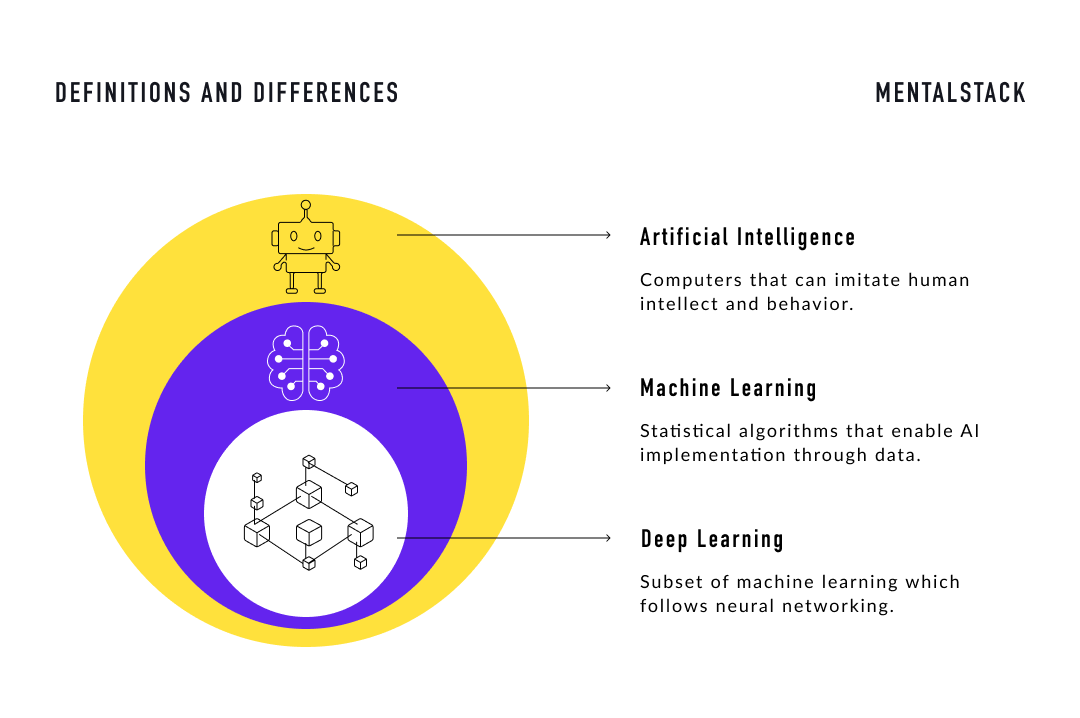
\includegraphics[width=\textwidth, height=\textheight, keepaspectratio]{ai-ml-dl.png}
  \end{center}
\end{frame}

\end{document}
